\section{Experiments} 
\label{sec:experiments}

All the pebbling algorithms and heuristics described in the previous sections have been implemented in the hybrid functional and object-oriented programming
language Scala (\url{www.scala-lang.org}) as part of the Skeptik library for proof compression (\url{github.com/Paradoxika/Skeptik}) \cite{Boudou}.

To evaluate the algorithms and heuristics, experiments were executed\footnote{The Vienna Scientific Cluster VSC\nobreakdash-2 
(\url{http://vsc.ac.at/}) was used.} on four disjoint sets of proof benchmarks (Table \ref{tab:benchmarks}). 
TraceCheck$_1$ and TraceCheck$_2$ contain proofs produced by the SAT-solver \texttt{PicoSAT} \cite{Biere2008} on unsatisfiable benchmarks from the SATLIB (\url{www.satlib.org/benchm.html}) library. 
The proofs\footnote{SAT proofs: \url{www.logic.at/people/bruno/Experiments/2014/Pebbling/tc-proofs.zip}} are in the TraceCheck proof format, which is one of the three formats accepted at the \emph{Certified Unsat} track of the SAT-Competition.
veriT$_1$ and veriT$_2$ contain proofs produced by the SMT-solver VeriT (\url{www.verit-solver.org}) on unsatisfiable problems from the SMT-Lib (\url{www.smtlib.org}). 
These proofs\footnote{SMT proofs: \url{www.logic.at/people/bruno/Experiments/2014/Pebbling/smt-proofs.zip}} are in a proof format that resembles SMT-Lib's problem format and they were translated into pure resolution proofs by considering every non-resolution inference as an axiom.

%%%%%%%%%%%%%%%%%%%%%%%%%%%%%%%%%%%%%%%%%%%%%%%%%%%%%%%%%%%%%%
%%%%%%%%%%%%%%% Benchmarks table &&&&&&&&&&&&&&&&&&&&&&&&&&&&&
%%%%%%%%%%%%%%%%%%%%%%%%%%%%%%%%%%%%%%%%%%%%%%%%%%%%%%%%%%%%%%

\begin{table}[tb]
	\centering
	\setlength{\tabcolsep}{8pt}
	\begin{tabular}{lrrr}
		\toprule
		%\textbf{Name} & \textbf{Number of proofs} & \textbf{Maximum length} & \textbf{Average length} \\ 
		\textbf{Name} & \textbf{Number of} & \textbf{Maximum} & \textbf{Average} \\ 
		              & \textbf{proofs}    & \textbf{length}  & \textbf{length} \\
		\midrule
		TraceCheck$_1$ & 2239 & 90756   & 5423   \\
		TraceCheck$_2$ & 215	& 1768249 & 268863 \\
    veriT$_1$ & 4187 & 2241042 & 103162 \\
    veriT$_2$ & 914  & 120075  & 5391  \\ 
		\bottomrule   
	\end{tabular}
	\caption{Proof benchmark sets}
	\label{tab:benchmarks}
\end{table}

%%%%%%%%%%%%%%%%%%%%%%%%%%%%%%%%%%%%%%%%%%%%%%%%%%%%%%%%%%%%%%
%%%%%%%%%%%%%%% Results table %%%%%%%%%%%%%%%%%%%%%%%%%%%%%%%%
%%%%%%%%%%%%%%%%%%%%%%%%%%%%%%%%%%%%%%%%%%%%%%%%%%%%%%%%%%%%%%
\begin{table}[tb]
\centering
%\setlength{\tabcolsep}{8pt}
\begin{tabular}{l c c}
\toprule
\textbf{Algorithm} & \textbf{Relative} & \textbf{Speed}\\ 
Heuristic & \textbf{Performance} (\%) & (nodes/ms)\\ 
\midrule

\textbf{Bottom-Up} & & \\
Children & 17.52 & \textbf{88.6} \\ 
LastChild & \textbf{26.31} & 84.5 \\ 
Distance(1) & 9.46 & 21.2 \\ 
Distance(3) & -0.40 & 0.5\\ 

\midrule

\textbf{Top-Down} & & \\
Children & -27.47 & 0.3 \\
LastChild & -31.98 & 1.9 \\
Distance(1) & -70.14 & 0.6 \\ 
Distance(3) & \textbf{-74.33} & \textbf{0.1}\\ 

\bottomrule
%\hline
\end{tabular}
\caption{Experimental results}
\label{tab:results}
\end{table}

\begin{table}[tb]
\centering
%\setlength{\tabcolsep}{8pt}

%%%%%%%%%%%%%%%%%%%%%%%%%%%%%%%%%%%%%%%%%%%%%%%%%%%%%%%%%%%%%%
%%%%%%%%%%%%%%% Decay table %%%%%%%%%%%%%%%%%%%%%%%%%%%%%%%%%%
%%%%%%%%%%%%%%%%%%%%%%%%%%%%%%%%%%%%%%%%%%%%%%%%%%%%%%%%%%%%%%

\begin{tabular}{c c c c c}
\toprule
\textbf{Decay} & \textbf{Depth} &  \textbf{Combination} & \textbf{Performance} & \textbf{Speed}\\ 
$\gamma$ &$d$ &  $com$ & \textbf{Improvement} (\%) & (nodes/ms)\\ 
\midrule
0.5&1& mean & 0.50 & 47.7\\ 
0.5& 1& maximum & 0.40 & 47.0 \\
0.5& 7& mean& 0.85 & 14.0 \\
0.5& 7& maximum & 0.76 & 15.3 \\
3&   1& mean & 0.48 & 64.0\\
3&   1& maximum & 0.43 & \textbf{64.4} \\
3&   7& mean & 0.21 & 15.3 \\ 
3&   7& maximum & \textbf{0.94} & 15.3 \\
\bottomrule
%\hline
\end{tabular}
\caption{Improvement of LastChild using Decay Heuristic}
\label{tab:decay}
\end{table}

Table \ref{tab:results} summarizes the results of the experiments.
The two presented algorithms are tested in combination with the four presented heuristics.
The Children and LastChild heuristics were tested on all four benchmark sets.
The Distance and Decay heuristics were tested on the sets TraceCheck$_2$ and veriT$_2$.
The relative performance is calculated according to Formula \ref{eq:space}, where $f$ is an algorithm with a heuristic, $P$ is the set of proofs the heuristic was tested on and $G$ are all combinations of algorithms and heuristics that were tested on $P$.
The time used to construct orders is measured in processed nodes per millisecond.
Both columns show the best and worst result in boldface.

\begin{align}
  \relPerfomance(f,P,G) = \frac{1}{|P|} * \sum_{\varphi \in P}{\left( 1 -
    \frac{
      s(\varphi,f(\varphi))
    }{
        \mathit{avg}_{g\in G}{s(\varphi,g(\varphi))}
    } \right)
  }
  \label{eq:space}
\end{align}

Table \ref{tab:results} shows that the Bottom-Up algorithm constructs topological orders with much smaller space measures than the Top-Down algorithm. 
This fact is visualized in Figure \ref{fig:BUvsTD}, where each point represents a proof $\varphi$.
The $x$ and $y$ coordinates are the smallest space measure among all heuristics obtained for $\varphi$ using, respectively, the Top-Down and Bottom-Up algorithm.
The results for Top-Down range far beyond 15000, but to display the discrepancy between the two algorithms the plot scales from 0 to 15000 on both axis.
The biggest best space measure for Top-Down is 131 451, whereas this number is 11 520 for the Bottom-Up algorithm.
The LastChild heuristic produces the best results and the Children heuristic also performs well.
The Distance heuristic produces the worst results, which could be due to the fact that the radius is too small for big proofs with thousands of proof nodes.

Table \ref{tab:decay} summarizes results of the Decay Heuristic with the best results highlighted in boldface.
Decay Heuristics were tested with the Bottom-Up algorithm, using LastChild as underlying heuristic.
For the parameters decay factor, recursion depth and combining function two values and all their combinations have been tested.
The performance improvement is calculated using Formula \ref{eq:space} with $G$ being the singleton set of the Bottom-Up algorithm with the LastChild heuristic.
The results show, that Decay Heuristics can improve the result, but not by a landslide.
The improvement comes at the cost of slower speed, especially when the recursion depth is big.

Some additional heuristics, not described in this work, designed specifically for Top-Down Pebbling were tested on small benchmark sets.
These heuristics aimed at doing local pebbling without having to calculate full spheres.
For example pebbling nodes that allow other nodes to be unpebbled in the next move can be preferred.
Unfortunately, none of the additional heuristics showed promising results.

%%%%%%%%%%%%%%%%%%%%%%%%%%%%%%%%%%%%%%%%%%%%%%%%%%%%%%%%%%%%%%
%%%%%%%%%%%%%%% Top-Down vs Bottom-Up figure %%%%%%%%%%%%%%%%%
%%%%%%%%%%%%%%%%%%%%%%%%%%%%%%%%%%%%%%%%%%%%%%%%%%%%%%%%%%%%%%

\begin{figure}
	\centering
	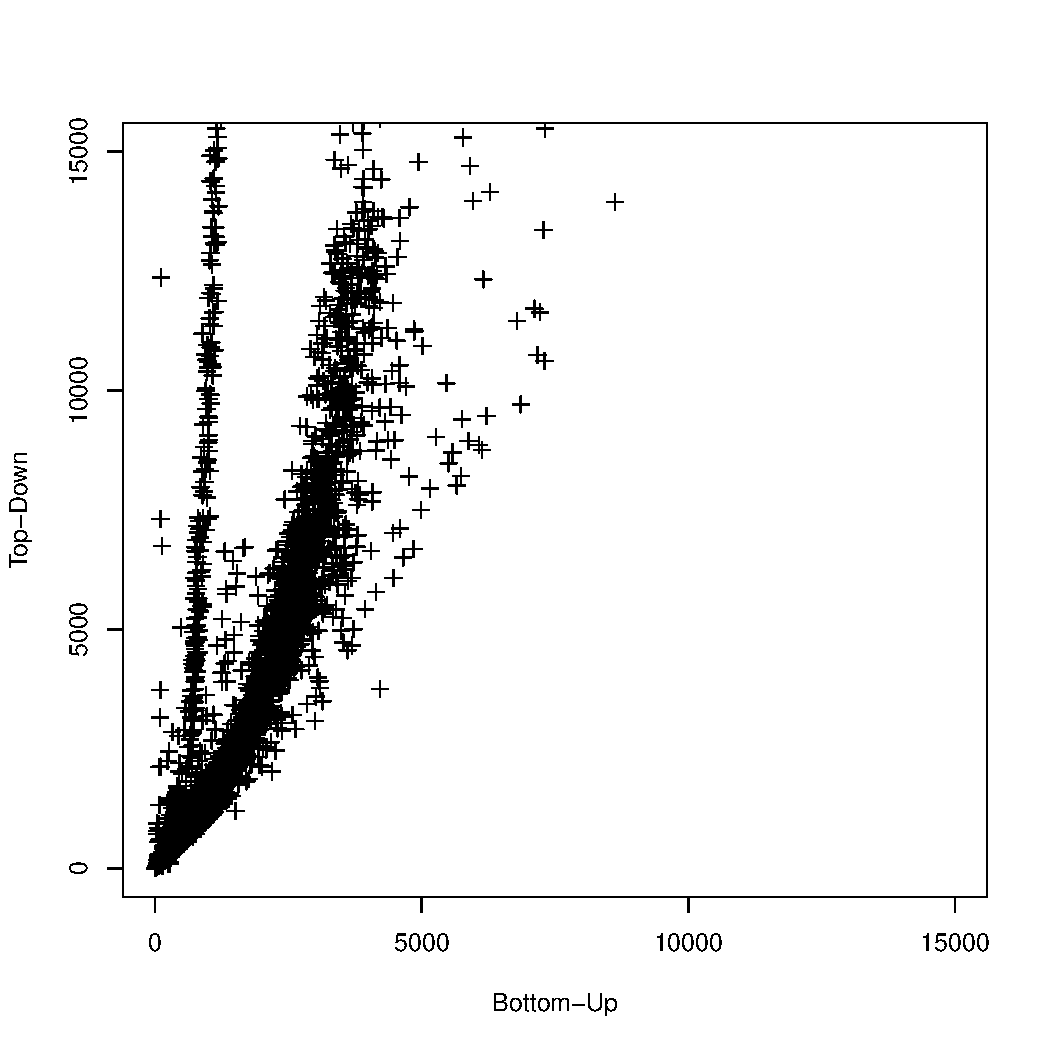
\includegraphics[scale=0.5]{chapters/pebbling/figures/td_vs_bu_2.pdf}
	\caption{Space measures of best Bottom-Up and Top-Down result}
	\label{fig:BUvsTD}
\end{figure}

The Bottom-Up algorithm does not only produce better results, it is also much faster, as can be seen in the last column of Table \ref{tab:results}. 
The reason probably is the number of comparisons that the algorithms make. 
For Bottom-Up the set $N$ of possible choices consists of the premises of a single node only, and usually $|N| \in O(1)$ (e.g. for a binary resolution proof, $N \leq 2$ always). 
For Top-Down the set $N$ is the set of currently pebbleable nodes, which can be large (e.g. for a perfect binary tree with $2n -1$ nodes, initially $|N| = n$). 
Possibly for some heuristics, Top-Down algorithms could be made more efficient by using, instead of a set, an ordered sequence of pebbleable nodes together with their memorized heuristic evaluations.

Unsurprisingly the radius used for the Distance Heuristic has a severe impact on the speed, which decreases rapidly as the maximum radius increases. 
With radius 5, only a few small proofs were processed in a reasonable amount of time.

On average the smallest space measure of a proof is 44.1 times smaller than its length. 
This shows the impact that the usage of deletion information together with well constructed topological orders can have. 
When these techniques are used, on average 44.1 times less memory is required for storing nodes in memory while proof processing.
